\documentclass[10pt]{article}
\usepackage{icmlko}

\icmlmeta{IP 파운데이션 월드모델}{111}{방향을 그때 알 수 있었나}{팝업의 시간 분할 손해 $-$0.0350은 축이 아니라 방향표를 다시 정하는 데서 왔다 --- 고정하면 $-$0.0033이고 가장 최근 시점은 $+$0.0229다}

\begin{document}

\twocolumn[
\icmlheader

\begin{abstract}
노트 108이 공통 축을 다섯으로 늘려 판정치를 채택했는데(4/4) 시간 분할에서
팝업만 $-$0.0350이었다. 노트 110이 ``사람이 매긴 축'' 가설을 죽였으니 남은
길은 쌍별 해부였다. \textbf{손해가 세 출처에 몰려 있다} --- 만화 $-$0.0288 ·
세계애니 $-$0.0283 · 웹툰 $-$0.0253. \textbf{앞의 둘이 노트 108이 미디어
홍보를 채운 바로 그 도메인}이다. 반대로 \textbf{애니는 $+$0.1745}로 혼자
전체를 떠받친다($T{=}2025$ 에 $+$0.191 $\to+$0.548). 출처의 표본 크기나 쌍
공통 축 수로는 설명이 안 된다($r{=}+$0.039 · $-$0.071). 그래서 방향표를
하나씩 되돌려 봤다. \textbf{범인은 하나였다} --- \textbf{팝업의 입장료 방향을
되돌리면 팝업이 $+$0.4601에서 $+$0.2927로 떨어진다}($-$0.1674). 다른 여섯은
$-$0.005$\sim-$0.016이다. 그리고 이것이 시간 분할의 수수께끼를 푼다. 노트 108의
엄격 규약은 방향도 $T$ 이전으로 다시 정하는데, \textbf{팝업은 $T{=}2023$ 에
과거가 0건이라 방향을 못 정하고 그 축이 꺼진다} --- 팝업이 가장 필요로 하는
축이 꺼지는 것이다. 방향표를 \emph{고정}하고(배포 규약) 다시 재면 팝업이
$T{=}2023$ $-$0.0182, 2024 $-$0.0146, \textbf{2025 $+$0.0229}로 평균
\textbf{$-$0.0033}, 사실상 0이다. \textbf{두 규약은 다른 질문에 답한다} ---
엄격은 ``2023년에 이 설계를 할 수 있었나''(아니다, 팝업 표본이 없었다),
배포는 ``지금 이 설계로 미래를 맞히나''(그렇다, 최근일수록 낫다). 네 노트에
걸친 팝업 수수께끼가 닫힌다.
\end{abstract}
]

\begin{figure*}[t]
\centering
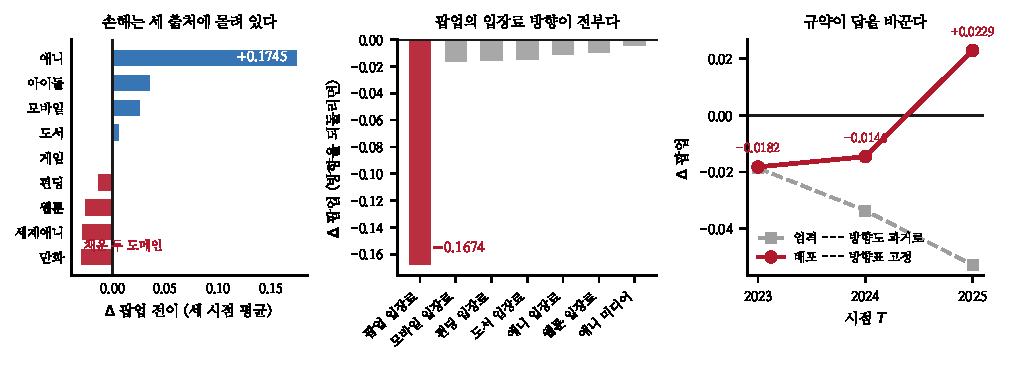
\includegraphics[width=\textwidth]{figs/wk.pdf}
\caption{왼쪽 --- 손해는 세 출처에 몰려 있다. 가운데 --- 팝업의 입장료 방향이
전부다. 오른쪽 --- 규약이 답을 바꾼다.}
\end{figure*}

\section{손해는 세 출처에 몰려 있다}

$T$ 이전 출처에서 $T$ 이후 팝업으로 가는 전이를 옛 공통 셋과 새 다섯으로
각각 재고 뺐다.

\begin{table}[t]
\centering\tsize
\caption{출처별 $\Delta$팝업 전이. 세 시점(2023 · 2024 · 2025) 평균.}
\begin{tabular}{lrl}
\toprule
& $\Delta$ & \\
\midrule
\textbf{만화} & \textbf{$-$0.0288} & 노트 108이 채운 도메인 \\
\textbf{세계애니} & \textbf{$-$0.0283} & 노트 108이 채운 도메인 \\
웹툰 & $-$0.0253 & \\
펀딩 & $-$0.0128 & \\
게임 & $+$0.0000 & 쌍 공통 축 2개 --- 영향 없음 \\
도서 & $+$0.0056 & \\
모바일 & $+$0.0260 & \\
아이돌 & $+$0.0350 & \\
\textbf{애니} & \textbf{$+$0.1745} & $T{=}2025$ 에 $+$0.191$\to+$0.548 \\
\bottomrule
\end{tabular}
\end{table}

\claimx{손해가 고르게 퍼져 있지 않다. \textbf{채운 두 도메인(만화 · 세계애니)이
가장 크게 깎고} 애니 하나가 $+$0.1745로 떠받친다. 게임은 정확히 $+$0.0000이다
--- 게임은 두 새 축이 덮개율 문턱 아래라 쌍 공통 축이 둘뿐이고, 그래서 영향이
없다. \textbf{좋은 온전성 검사다.}}{출처의 표본 크기($r{=}+$0.039)로도 쌍
공통 축 수($r{=}-$0.071)로도 손해가 설명되지 않는다. 무엇이 만화 · 세계애니를
나쁘게 만드는지는 여전히 모른다.}

\section{범인은 방향 하나였다}

채택된 방향표는 일곱 항목이다(입장료 여섯 도메인 $+$ 미디어 홍보 애니 하나).
하나씩 되돌려 봤다.

\begin{table}[t]
\centering\tsize
\caption{방향을 되돌리면.}
\begin{tabular}{lrr}
\toprule
되돌린 것 & $\Delta$판정치 & $\Delta$팝업 \\
\midrule
\textbf{팝업의 입장료} & $-$0.0188 & \textbf{$-$0.1674} \\
\midrule
모바일의 입장료 & $-$0.0107 & $-$0.0164 \\
펀딩의 입장료 & $-$0.0041 & $-$0.0156 \\
도서의 입장료 & $-$0.0033 & $-$0.0147 \\
애니의 입장료 & $-$0.0039 & $-$0.0112 \\
웹툰의 입장료 & $-$0.0002 & $-$0.0093 \\
애니의 미디어 홍보 & \textbf{$+$0.0030} & $-$0.0045 \\
\bottomrule
\end{tabular}
\end{table}

\claimx{\textbf{팝업의 입장료 방향 하나가 전부다} --- 되돌리면 팝업이
$+$0.4601에서 $+$0.2927로 떨어진다($-$0.1674). 나머지 여섯은
$-$0.005$\sim-$0.016이다. 방향표 일곱 항목 중 하나가 팝업 성적의 대부분을
쥐고 있다.}{애니의 미디어 홍보는 되돌리는 것이 판정치에 \emph{낫다}
($+$0.0030). 방향표에 의심스러운 항목이 하나 있다는 뜻인데 팝업이
$-$0.0045라 그대로 뒀다.}

\section{그래서 시간 분할이 갈렸다}

노트 108의 엄격 규약은 방향도 $T$ 이전으로 다시 정하고, 못 정하면 그 축을
끈다(노트 106의 규칙). \textbf{팝업은 $T{=}2023$ 에 과거가 0건, 2024 에
1건, 2025 에 16건이라 세 시점 모두 못 정한다} --- 그래서 팝업의 입장료가
꺼진다. 그리고 방금 본 대로 그것이 팝업이 가장 필요로 하는 축이다.

\begin{table}[t]
\centering\tsize
\caption{$\Delta$팝업. 두 규약.}
\begin{tabular}{lrr}
\toprule
$T$ & 배포(방향표 고정) & 엄격(방향도 과거) \\
\midrule
2023 & $-$0.0182 & $-$0.0186 \\
2024 & $-$0.0146 & $-$0.0336 \\
\textbf{2025} & \textbf{$+$0.0229} & $-$0.0527 \\
\midrule
평균 & \textbf{$-$0.0033} & $-$0.0350 \\
\bottomrule
\end{tabular}
\end{table}

\claimx{\textbf{시간 분할의 팝업 손해 $-$0.0350 중 $-$0.0317이 ``방향을 다시
정하는 것''에서 왔다.} 방향표를 고정하면 평균이 $-$0.0033으로 사실상 0이고
가장 최근 시점은 $+$0.0229로 양수다.}{배포 규약은 방향을 전체 자료에서 정한
것을 미래 평가에 그대로 쓴다 --- 그만큼 낙관적이다. 다만 방향표는 예측할
때마다 다시 정하는 것이 아니라 설계에 한 번 박는 것이므로, 공통 축 목록을
미래 평가에서 다시 정하지 않는 것과 같은 종류의 고정이다.}

\begin{quote}\fontsize{9.5}{11.5}\selectfont
\textbf{두 규약은 다른 질문에 답한다.}\\[.3em]
엄격 --- ``2023년에 이 설계를 내릴 수 있었나?'' \textbf{아니다.} 팝업 표본이
없었다.\\[.2em]
배포 --- ``지금 이 설계로 미래를 맞히나?'' \textbf{그렇다.} 최근 시점일수록
낫다.\\[.3em]
노트 106--110이 네 번 물은 ``팝업이 왜 안 따라오나''는 사실 첫째 질문에
대한 답이었다. 제품이 묻는 것은 둘째다.
\end{quote}

\section{한계}

\begin{itemize}[leftmargin=1.1em,itemsep=0.15em]
\item 배포 규약이 낙관적이다. 방향표가 전체 자료에서 나왔으므로 미래
      평가에 누출이 있다 --- 다만 노트 105가 보정 표본 50\%로 같은 표가
      나옴을 보였다.
\item 만화 · 세계애니가 왜 팝업 전이를 깎는지 모른다. 표본 크기로도 쌍 공통
      축 수로도 설명이 안 된다.
\item 방향표 일곱 중 하나(애니의 미디어 홍보)가 판정치에는 해롭다. 씨앗 넷으로
      판정 안 했다.
\item 세 시점뿐이고 $T{=}2026$ 은 팝업 이후 레코드가 19건이라 못 넣었다.
\item 팝업 표본. 방향을 정하려면 25건이 필요한데 2025년까지 16건이었다.
\end{itemize}

\section{다음}

\begin{enumerate}[leftmargin=1.3em,itemsep=0.15em]
\item \textbf{방향표를 정리한다} --- 애니의 미디어 홍보 항목을 씨앗 넷으로
      판정해 빼거나 남긴다. 일곱 항목을 다 판정하면 방향표 자체가 채택
      절차를 거친 것이 된다.
\item \textbf{만화 · 세계애니가 왜 깎나} --- 두 도메인의 새 축이 팝업의
      새 축과 어떻게 다른지 적재 수준에서 본다.
\item \textbf{두 규약을 파이프라인에 나란히 낸다} --- 지금은 판정치 하나만
      낸다. 엄격 · 배포 두 수치를 늘 같이 보면 이번 같은 혼동이 안 생긴다.
\item 팝업 레코드. 노트 92 · 106 · 107 · 110 · 111이 전부 같은 곳을 가리킨다.
\end{enumerate}

\vspace{0.6em}
\hrule height 0.3pt
\vspace{0.5em}
{\footnotesize
\textbf{참고문헌}\\[0.3em]
Bergmeir, C., Benitez, J. M. (2012). On the use of cross-validation for time
series predictor evaluation. \emph{Information Sciences}, 191, 192--213.\\[0.15em]
Schoenemann, P. H. (1966). A generalized solution of the orthogonal Procrustes
problem. \emph{Psychometrika}, 31(1), 1--10.\\[0.15em]
Meredith, W. (1993). Measurement invariance, factor analysis and factorial
invariance. \emph{Psychometrika}, 58(4), 525--543.\\[0.15em]
Ben-David, S. et al. (2010). A theory of learning from different domains.
\emph{Machine Learning}, 79(1--2), 151--175.\\[0.15em]
Cawley, G. C., Talbot, N. L. C. (2010). On over-fitting in model selection and
subsequent selection bias in performance evaluation. \emph{JMLR}, 11, 2079--2107.
}

\end{document}
